\setcounter{page}{1}
\section*{Zielsetzung}

In dem Versuch V703 sollen die Charakteristika eines %würde den Begriff Charakteristika nicht benutzen, weil er in dem Zusammenhang schon reserviert ist
Geige-Müller-Zählrohr untersucht werden, zu diesen gehören die %Geiger-Müller-Zählrohrs, Punkt statt Komma
Totzeit und die Untersuchung von Nachentladungen. %so klingt es, als sei die Untersuchung eine Charakteristik

\section{Theorie}

\subsection{Funktionsweise eines Geiger-Müller-Zählrohr}
Ein Geiger-Müller-Zähler besteht grundsätzlich aus einem %grundsätzlich unpassend
Kathodenzylinder (negativ geladen) und einem Anodendraht (positiv geladen) (vgl. Abbildung \ref{fig: schematischer_aufbau}).
Zwischen Anode und Kathode befindet sich ein Gasgemisch (bestehend aus einem Edelgas
und Alkohldampf).
\begin{figure}
  \centering
  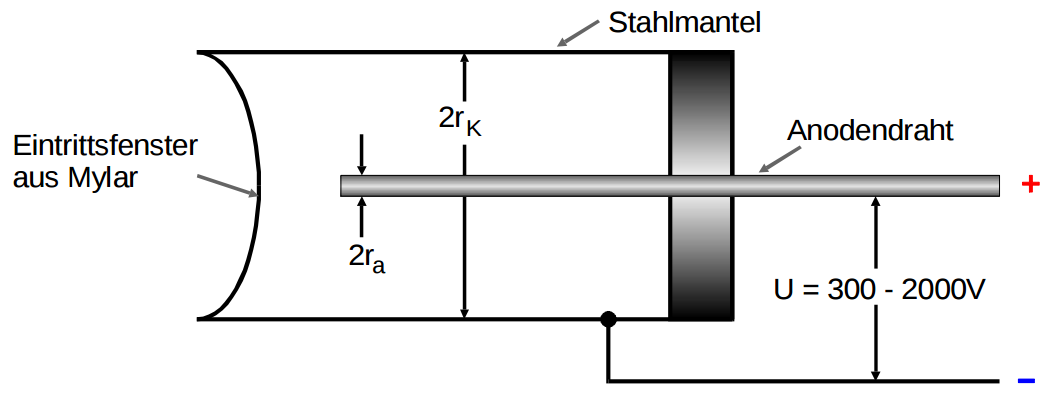
\includegraphics[width=0.6\textwidth]{bilder/geiger_.png}
  \caption{Schematische Darstellung eines Geiger-Müller-Zählrohrs \cite{anleitung703}.}
  \label{fig: schematischer_aufbau}
  \end{figure}
Durch Anlegen einer Spannung ($300-\SI{2000}{\volt}$) entsteht ein elektrisches
Feld Inneren des Zylinders. Auf der Vorderseite des Geiger-Müller-Zählrohrs %im Inneren
befindet sich ein Eintrittsfenster aus Mylar. Dieses ermöglicht es selbst $\alpha$- %Mylar ist nicht das Material
Strahlung in das Zählrohr einzutreten. %Grammatik

Gelangt ionisierende Strahlung in das Zählrohr, so ionisiert diese das Gasgemisch. %redundant
Die freigeschlagenen Elektronen können je nach anliegender Spannung, weitere Atome ionisieren. %entweder keine Kommas oder noch ein nach können
Die dadurch entstehende Elektronenlawine (als Townsend-Lawine bezeichnet) gelangt zu der Anode und erzeugt so
einen Strom. Der Strom wird mittels einem Verstärker verstärkt und an ein %redundant; mittels eines
Zählgerät weitergeleitet.

Wie oben angesprochen hängt die Anzahl der registrierten
Elektronen von der anliegenden Spannung ab (vgl. Abbildung \ref{fig:teilchen_spannung}).
\begin{figure}
  \centering
  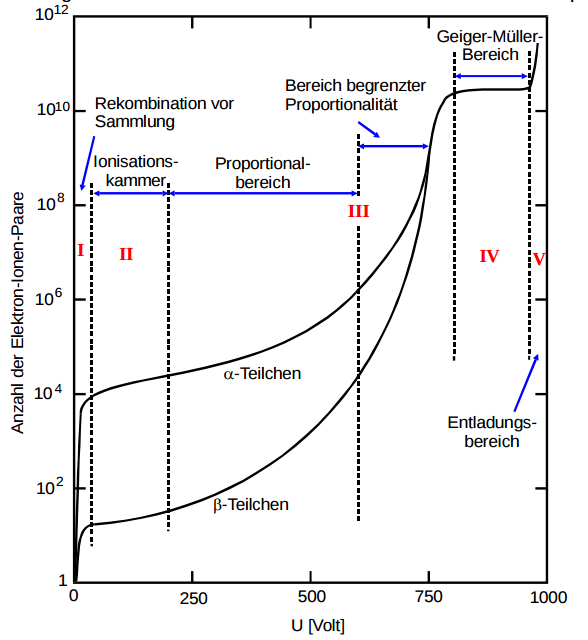
\includegraphics[width=0.6\textwidth]{bilder/diagramm.png}
  \caption{Anzahl der gemessen Teilchen pro Zeit bei unterschiedlichen Spannugen \cite{anleitung703}.} %Spannungen
  \label{fig:teilchen_spannung}
\end{figure}
Auf Grund der zu geringen Spannung gehen die meisten Elektronen durch Rekombination verloren. Dreht man die Spannung weiter auf,
kommt man in den \emph{Arbeitsbereich einer Ionisationskammer}, dieser funktioniert aber nur bei
Strahlungen mit hoher Intensität. Durch eine weitere Erhöhung der Spannung gelangt man
in den sogenannten \emph{Propotionalbereich}. In diesem besitzen die Elektronen
genügend Energie, um ihrerseits weitere Atome ionisieren zu können (auch Stoßionisation genannt).
Der Vorteil des Bereiches liegt daran, dass hier neben der Teilchenanzahl auch die Energie %darin
einfallender Teilchen gemessen werden kann. Bei wiederholte Erhöhung der Spannung %wiederholter
gelangt man in den \emph{Auslösebereich}. Hier liegt der Arbeitsbereich des
Geiger-Müller-Zählers.In diesem Spannungsbereich enthalten die ausgelösten Elektronenlawinen %Leerzeichen nach punkt
eine große Anzahl an UV-Photonen. Die Photonen können sich senkrecht zum elektrischen Feld bewegen
und lösen so Townsend-Lawine im gesamten Zählrohr aus. %lawinen, überarbeite die Formulierungen in diesem Absatz

Das Auftreten der Elektronlawinen im ganzen Rohr, hat eine \emph{Totzeit} zu folge, %kein Komma
bei dieser ist es dem Zählrohr nicht möglich neu eindringende Teilchen %bei dieser falsch
zu messen. Begründen kann die Unempfindlichkeit mit die durch die Elektronenlawine entstehenden %kann man; mit den; Satz überarbeiten
positiv geladenen Ionen. Da die Ionen eine größere Masse als Elektronen besitzen,
bewegen sie sich wesentlich langsamer zur Kathode, als die Elektronen
zur Anode. Dadurch entsteht in der Kammer ein Gegenfeld, welches das
elektrische Feld (erzeugt von Kathode und Anode) abschwächt.
Erst nachdem die Ionen die Kathode erreicht haben, ist eine
Registrierung wieder möglich. Nach der Totzeit schließt sich
noch eine \emph{Erholungszeit} an. In dieser Zeit erzeugen
die an der Kathode eintreffenden Ionen neue Elektronen, die eine neue
schwächere Elektronenlawine herrvorufen können (Nachentladung gennant). Beide Zeiten sind %hervorrufen; genannt
in Abbildung \ref{fig: tot_und_erholungszeit} grafisch dargestellt.
\begin{figure}
  \centering
  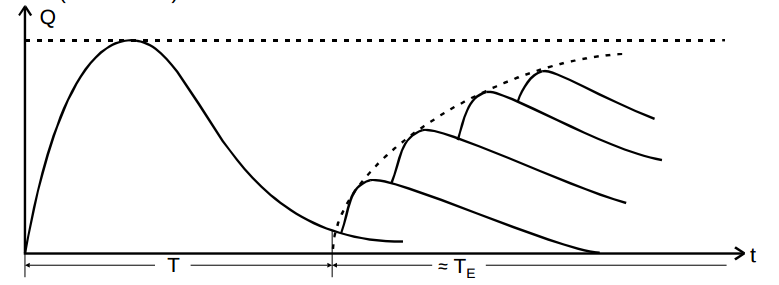
\includegraphics[width=0.6\textwidth]{bilder/totzeit.png}
  \caption{Grafische Darstellung von Tot- und Erholungszeit \cite{anleitung703}.}
  \label{fig: tot_und_erholungszeit}
  \end{figure}

Der Alkoholdampf im Gasgemisch soll die Erholungszeit verringern. Erklärbar ist es damit, dass %Erklärbar ist es damit klingt doof
die Edelgasionen die Alkoholmoleküle ionisieren. Die Alkoholmoleküle
besitzen eine geringere Ionisierungsenergie und können so keine Elektronen aus
der Kathode schlagen. Zusätzlich besitzt sie mehr Schwingungsmodie %moden (kein modus)
mit unterschiedlichen Frequenzen. Dadurch verliert das Alkohlmolekül %Alkohol
weiter Energie (wegen $E=\map{h}f$). %wegen doof

\subsection{Charakteristika des Zählrohrs}
In dem Arbeitsbereich des Geiger-Müller-Zählers erhält man einen
charakteristischen Verlauf für die regrestierten Teilchen $N$ in Abhängigkeit zur Spannung. %regestrierten, in der Anleitung und in der Auswertung ist N die Zählrate
Diese \emph{Charakteristik} ist in Abbildung \ref{fig: plateau} dargestellt.
\begin{figure}
  \centering
  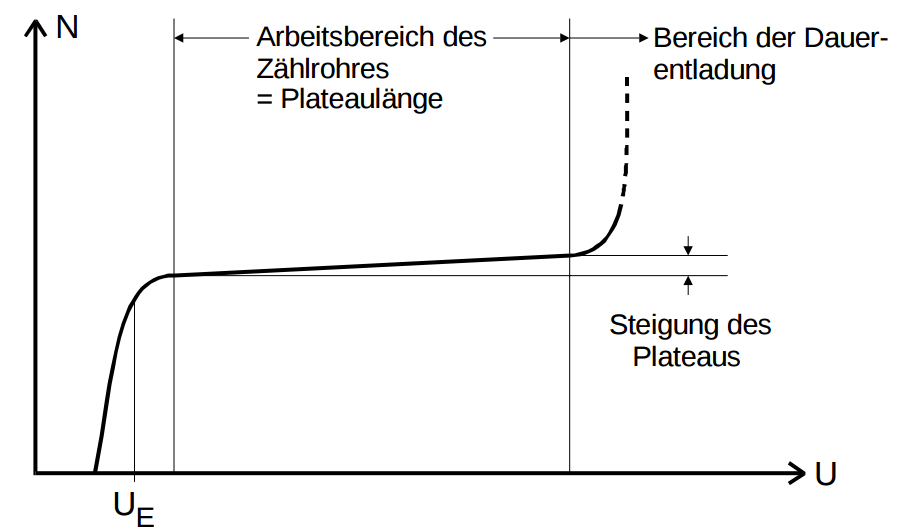
\includegraphics[width=0.6\textwidth]{bilder/pleateu.png}
  \caption{Vergrößerung des Geige-Müller-Bereichs \cite{anleitung703}.}
  \label{fig: plateau}
\end{figure}
Ab der Spannung $U\ua{E}$ erreicht man den idealen Spannungsbereich das Zählrohr. %rohrs
Für Spannungen größer als $U\ua{E}$ ist ein
linearer Zusammenhang zwischen $N$ und $V$ erkennbar, dieser Bereich wird auch als
\emph{Plateau} bezeichnet. Bei einem idealen Zählrohr besitzt der
lineare Zusammenhang eine Steigung von null. In der Realität jedoch besitzt
die Gerde eine geringe Steigung. Erklärbar ist die Steigung mit den oben angesprochenen Nachentladungen. %Gerade
Am Ende des Plateau nimmt die
Zahl der Nachentladungen gewaltig zu. Wird die Spannung hier noch weiter erhöht, %gewaltig umgangssprachlich
ist eine Zerstörung des Zählrohrs möglich.

%Überarbeite die Theorie nochmal, viele Sätze sind unschön/unpräzise formuliert
